Hotspotizer has been developed through a user-centered design process, in order to fulfill the needs of end-users. This section describes the evolution of Hotspotizer, the evaluation of the final prototype, and insights gained throughout development and deployment.

\section{Formative Studies}
\label{sec:formative-studies}

In the early stages of the design work for a tool to support authoring mid-air gestural interactions, the motivating question was \emph{what} to build. Design efforts were guided largely by qualitative and semi-structured feedback from users and inspiration from related work. Many concepts, in the form of rough sketches and paper prototypes, were produced. Concepts at this early stage included an end-to-end environment for creating gesture-controlled interactive movies that fused gesture authoring and content creation in one application; ready-made widgets that pre-implemented gesture control and plugged into existing development and design environments; and tools to overlay information (such as the distance between two specific joints) onto a visualization of a skeletal model, to complement textual programming.

The rough sketches, paper prototypes and mockups have been presented at a workshop to a group of 10 potential users, aged 22-31 ($\mu$=26), from diverse backgrounds. While recruited from among students and staff of a single university and not representative of a wide demographic, the participants represented the target users of Hotspotizer well. Each had different skills and interests. Among them was an industrial designer, a semi-professional musician, an electronics engineer, a computer scientist, a museum studies student, an interaction designer, a psychologists and a legal consultant. After a presentation on current design tools for mid-air gestural interfaces and our concepts, we collected feedback and made note of new ideas. Although all of the users were self-reportedly familiar with mid-air gestural interaction in the context of gaming, none had any familiarity with existing tools for authoring custom interfaces. Discussions on possible applications for custom gesture control revealed that a modular approach that can interface with a diverse variety of applications is preferable to a full-blown content creation suite. Moreover, even among users engaged in design or programming activities, tools used for these purposes varied greatly. This illustrated the value of a standalone application rather than a tool that generates code in a specific programming language or plugs into a specific environment.

Another round of sketches and prototypes was prepared, some of them higher fidelity, such as a mock screencast showing the use of various modules in a gesture authoring suite. The idea of creating virtual buttons or hotspots in the space around the user and using them to define gestures was depicted in the sketches, as well as an interactive mockup developed in Processing\footnote{\href{http://processing.org/}{processing.org}} (see Figure~\ref{fig:sketches-prototypes}). Other ideas included an application that recognized static poses and a graphical language consisting of atomic primitives for composing gestures. These were presented at a second workshop with the same 10 participants. Here, the concept of space discretization was proposed by a participant, an interaction designer. Upon interacting with the mockup of an interface where free-form areas in space can be made into gesture-tracking hotspots, she commented that she often makes use of squared paper when sketching. Instead of defining free-form regions in space, why not divide space into squares and constrain hotspots to these squares? Further discussion with participants revealed that this paradigm is grasped more easily than composing with atomic actions or constraints, or even demonstration. Moreover, using a visualization of the skeletal model and the space around it allows direct manipulation \parencite{Hutchins:1985}; encapsulates the limitations and prospects of the design space; capitalizes on proprioception; and can mediate interaction through a tight feedback loop \parencite{Wilson:2012}.

\begin{figure}[ht]
\centering
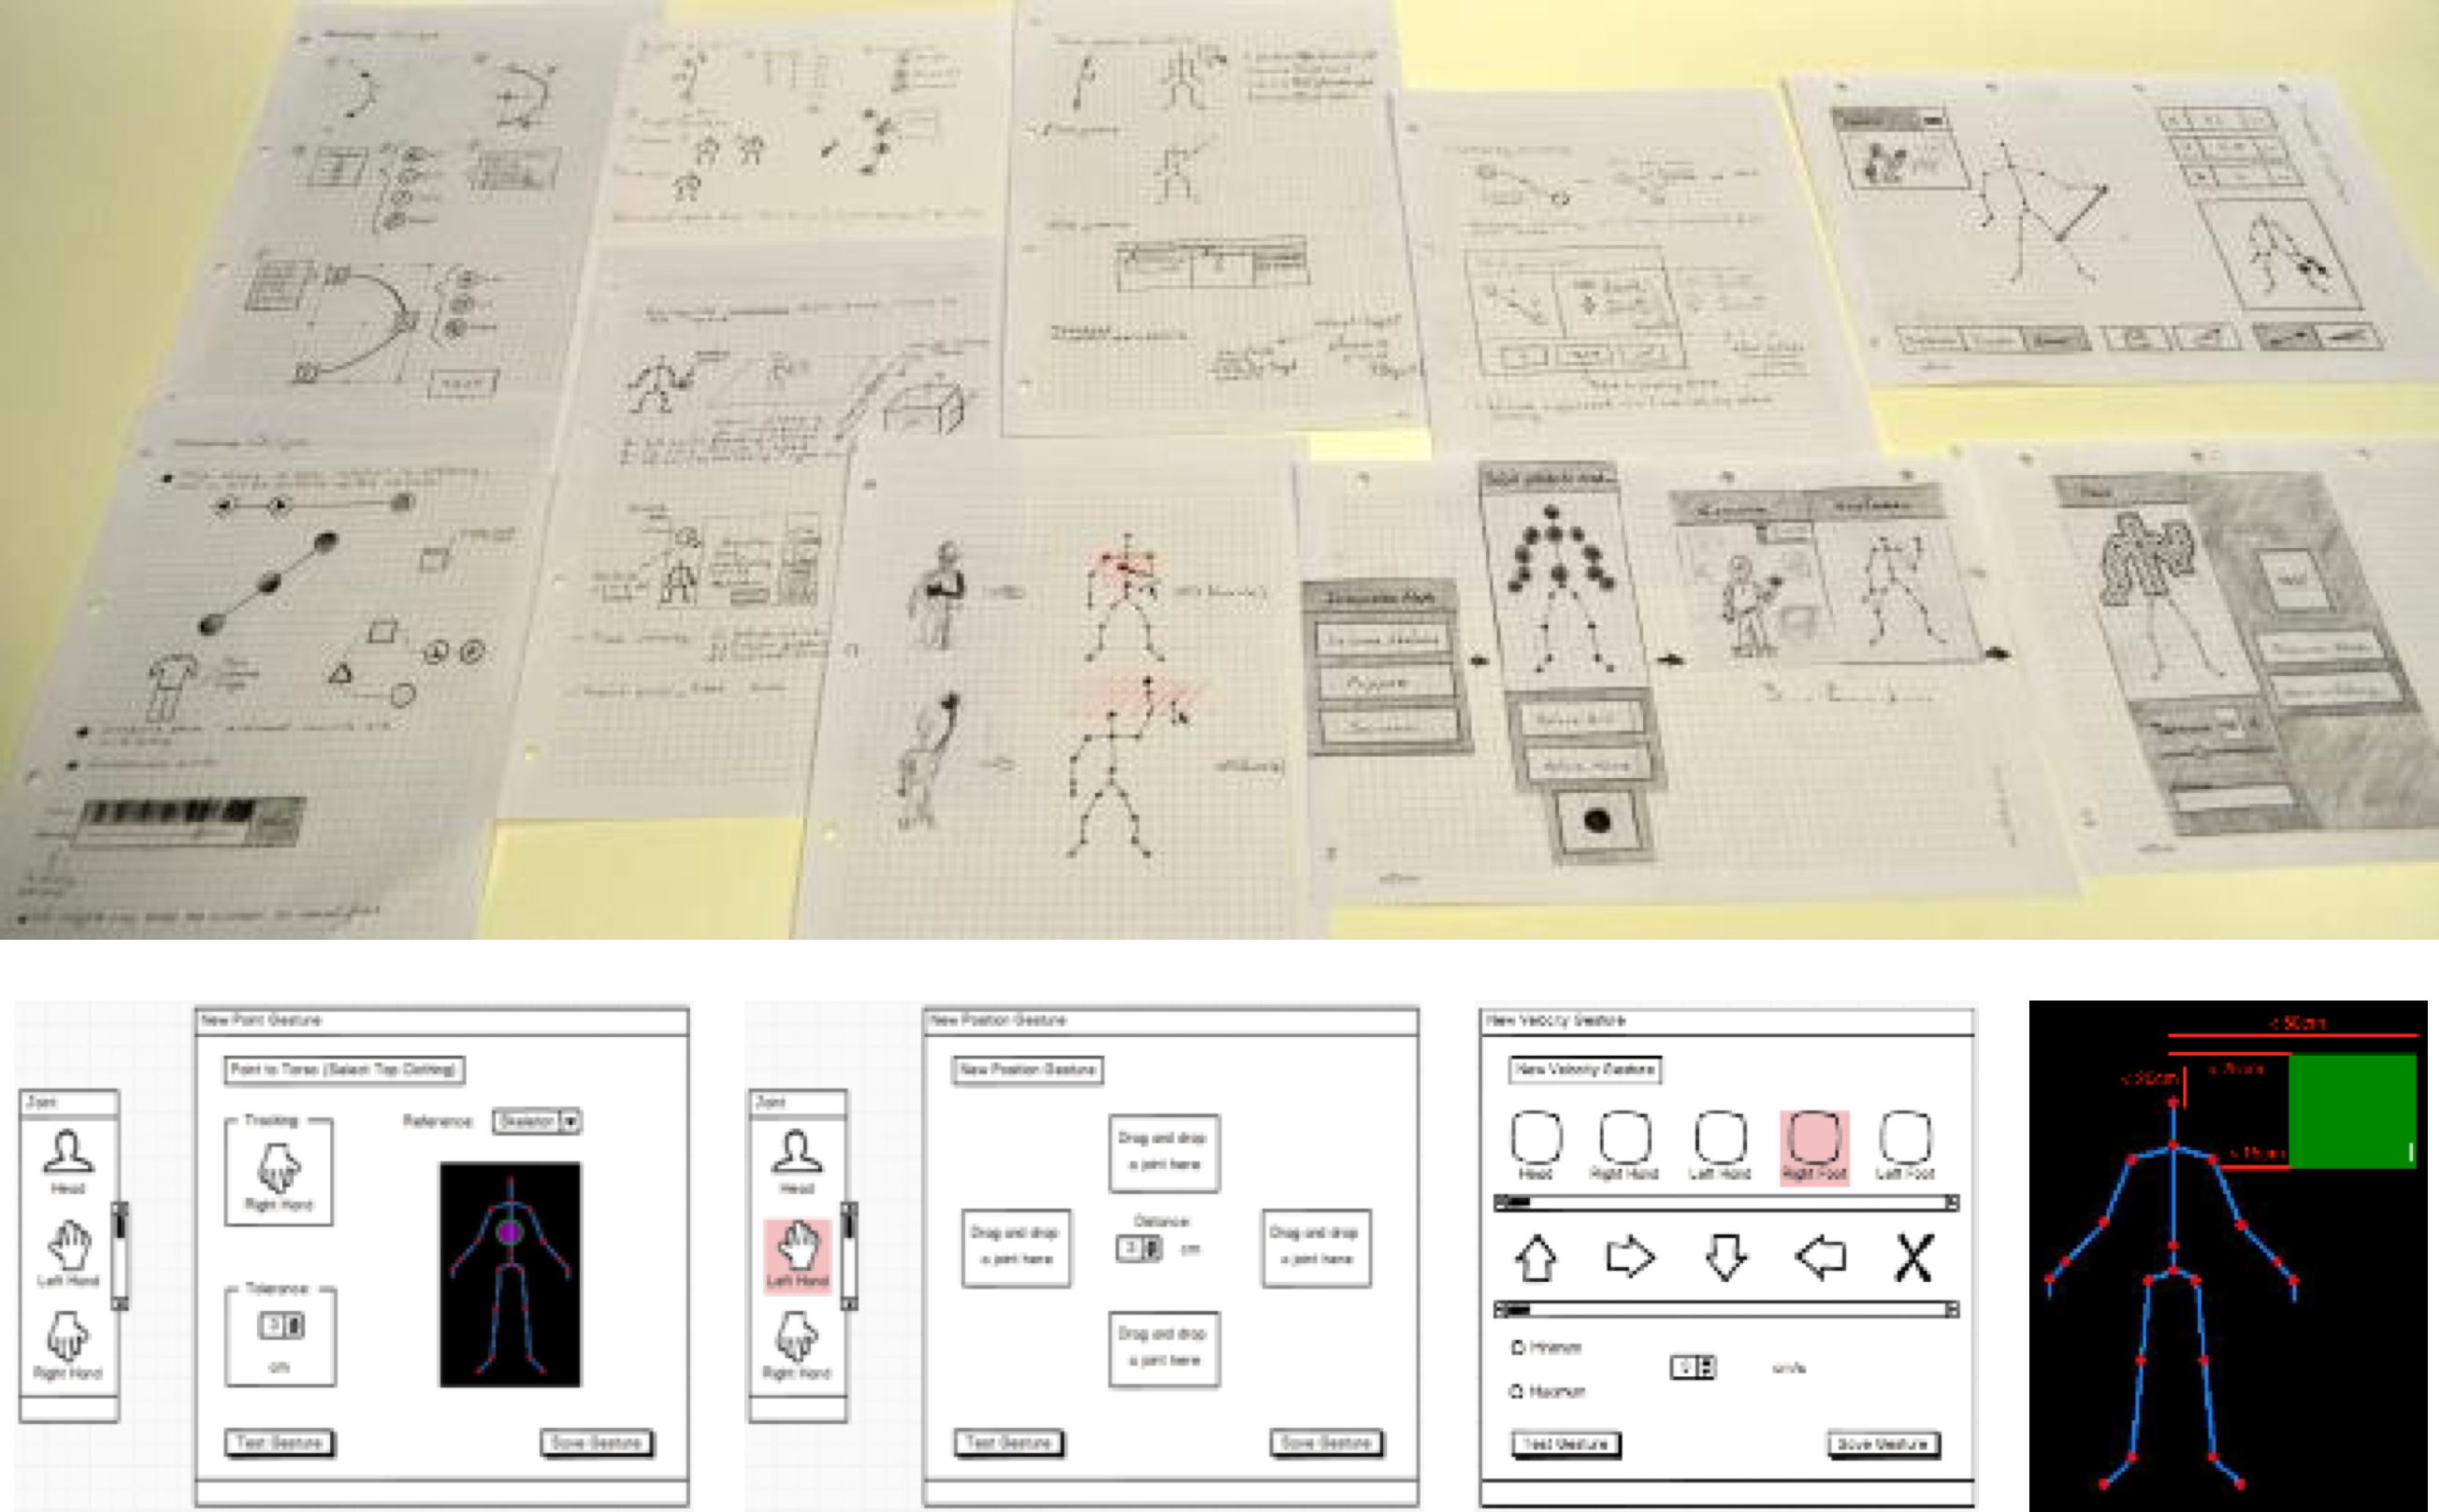
\includegraphics[width=\textwidth]{sketches-prototypes}
\caption{Rough sketches, paper prototypes and mockups were used to gather feedback which directed design and development.}
\label{fig:sketches-prototypes}
\end{figure}

Hotspotizer was developed as an implementation of this \emph{space discretization} paradigm yielded by these workshops. The design guidelines derived from \textcite{Olsen:2007} and \textcite{Shoemaker:2010} were used as filters that transformed the findings from the formative studies into a concrete user interface design. The decision to map gestures to key press events from an emulated keyboard was grounded in \posscite{Olsen:2007} principle for building on an infrastructure that is common across users and situations.

\section{Summative Studies}
\label{sec:summative-studies}

To evaluate Hotspotizer in use, two studies were conducted. The first was a study with 5 users to assess if Hotspotizer conforms to its design rationale. The second was a class workshop with 6 students working in pairs to build interactive prototypes of gestural interfaces. Qualitative results from these summative studies confirm that Hotspotizer conforms to our design rationale (see Figure~\ref{fig:design-guidelines-satisfied} for a summary of the observations that relate to the design guidelines).

\begin{SCfigure}[\sidecaptionrelwidth][ht]
\centering
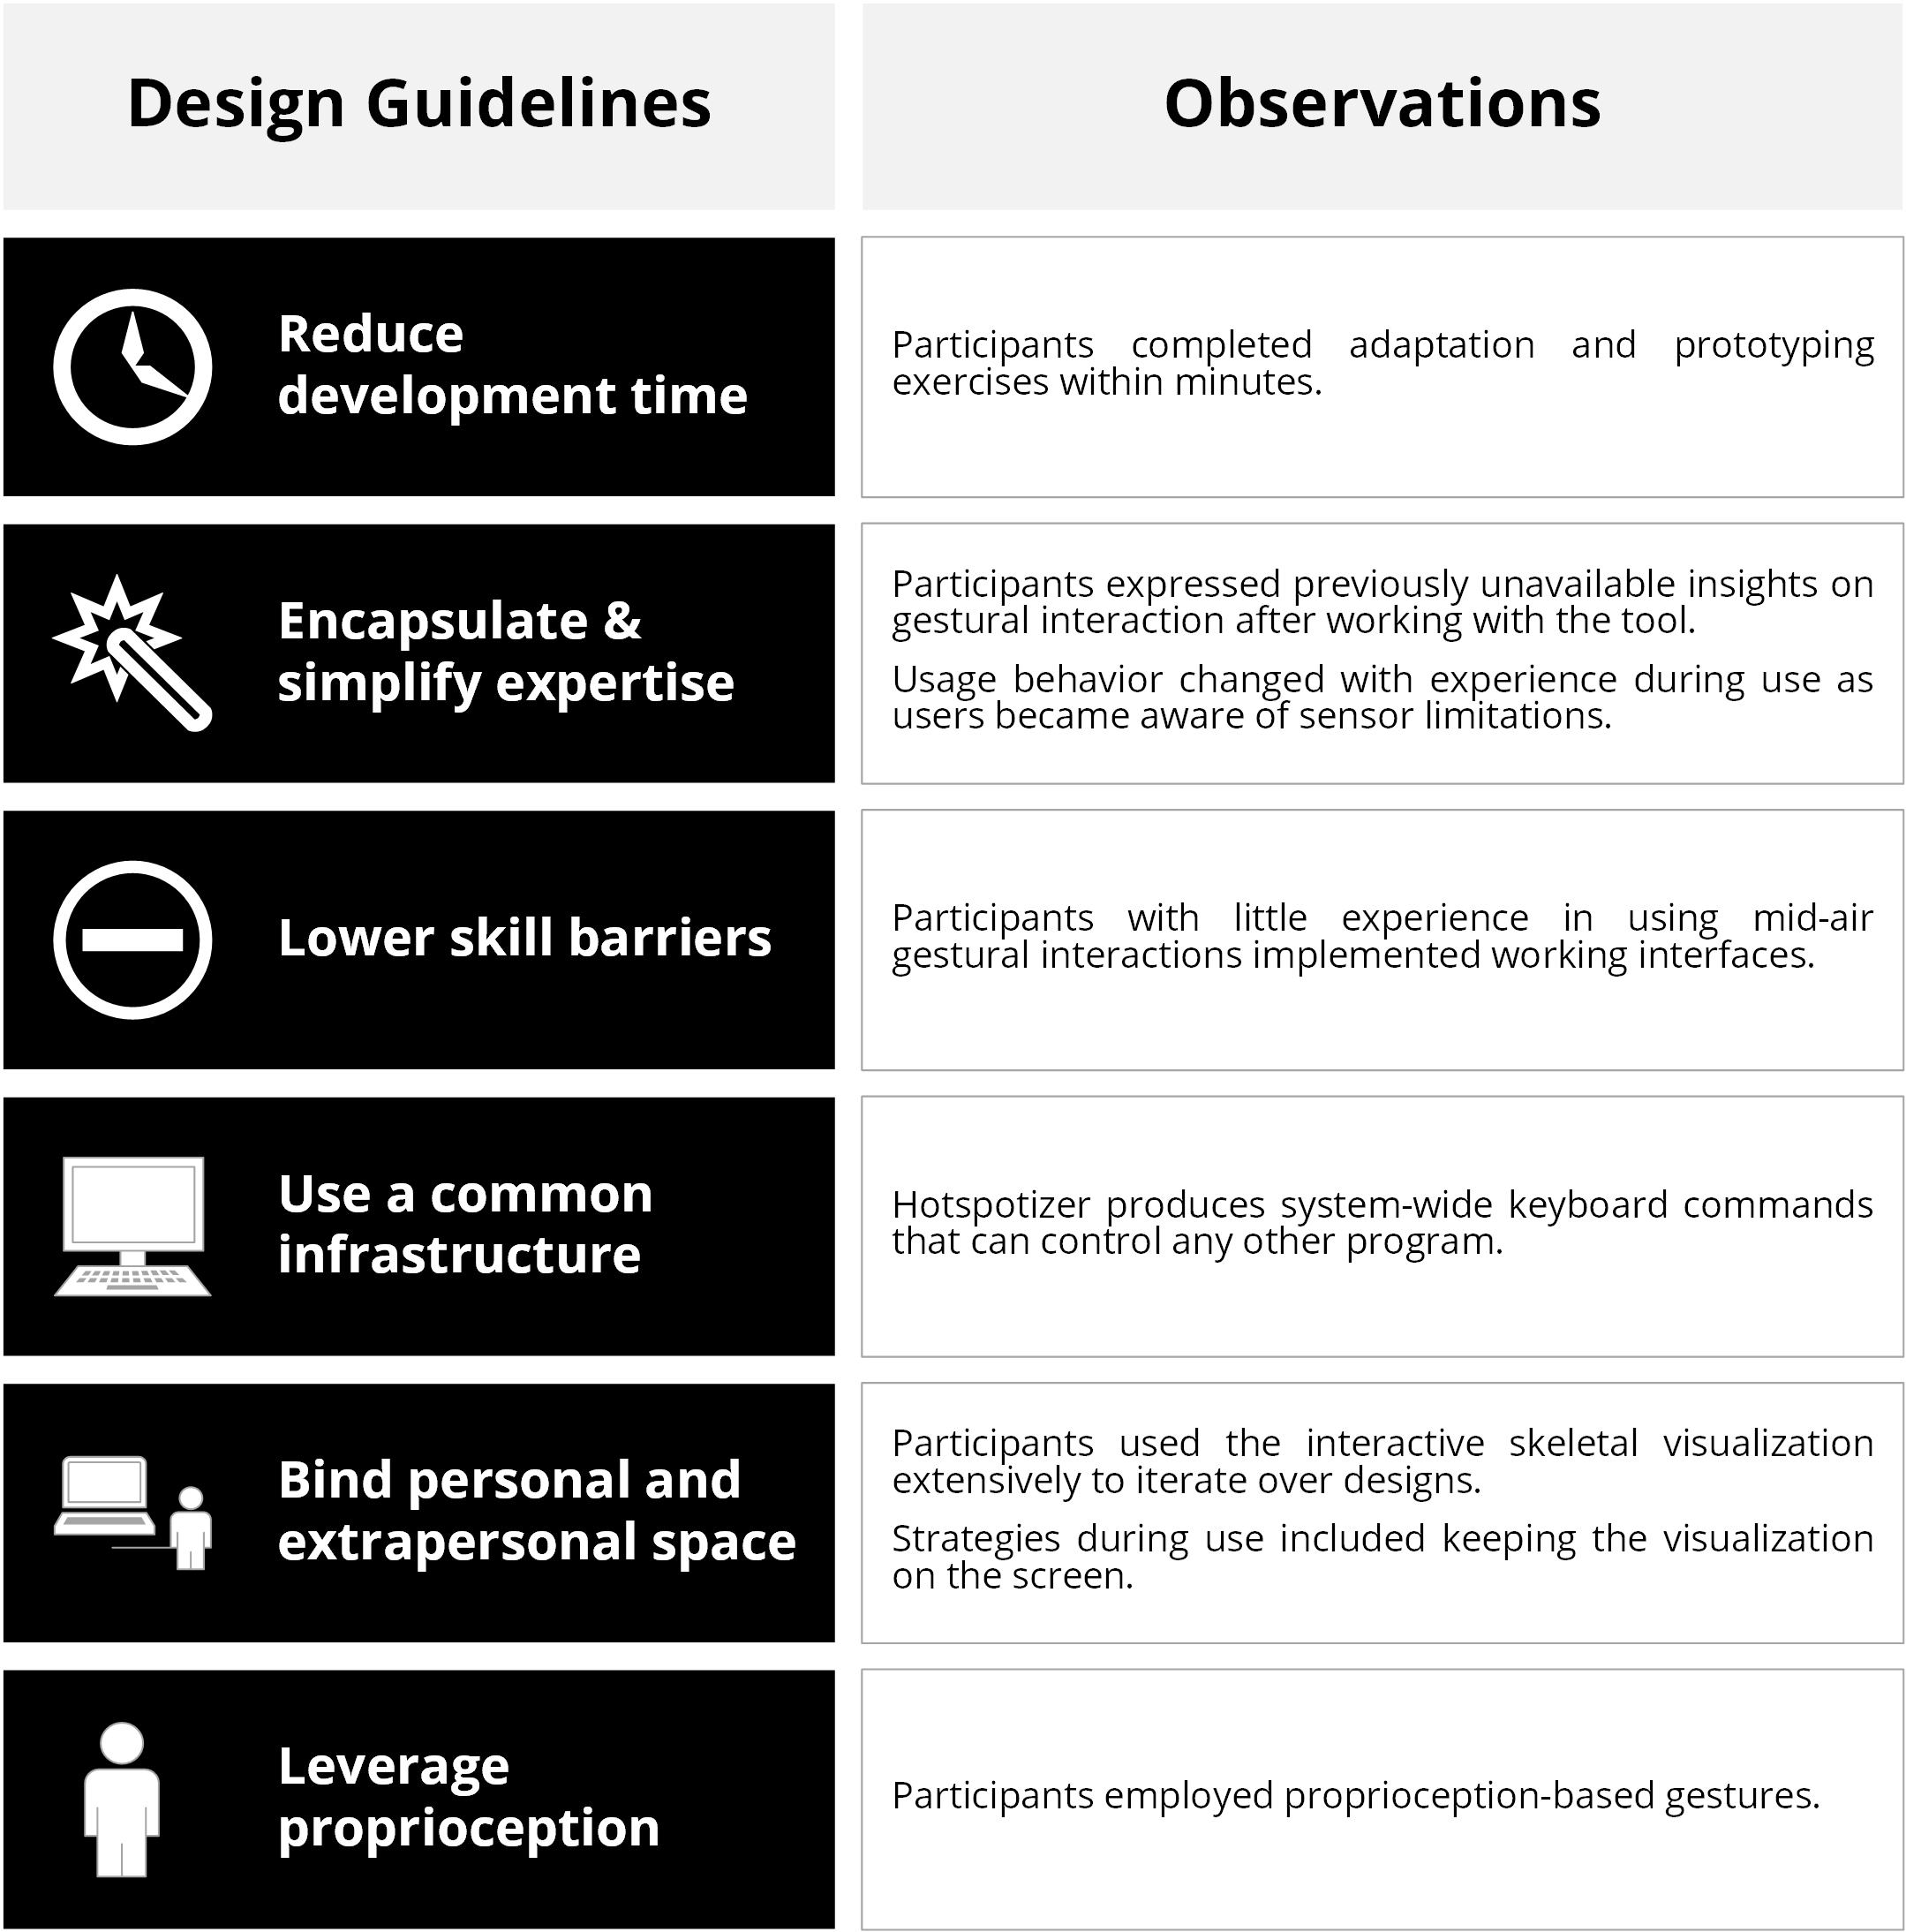
\includegraphics[width=.7\textwidth]{design-guidelines-satisfied}
\caption{Qualitative findings from two studies affirm that Hotspotizer is in keeping with our design rationale.}
\label{fig:design-guidelines-satisfied}
\end{SCfigure}

\subsection{User Study}

For the user study, five graduate students were recruited: an industrial designer, a museum studies student, a computer scientist, a psychologist and an interaction designer. These were not the same people who participated in the previous workshops. Participants were given a pre-study questionnaire where, on average, they self-reported a low level of experience with computer programming ($\mu$=2.1 on a 5-point Likert scale) and a low-medium level of experience with using mid-air gesture-based interfaces ($\mu$=2.4).

Participants were given the task of adapting a non-gestural interface for a computer game to gesture control. They were provided a PC with a Kinect sensor. The game was a side-scrolling platformer --- this style of game was selected since users were expected to be fully familiar with the game mechanics and not be distracted from the process of gesture authoring. The participants were not given specific gestures to implement, but the game required three commands to operate: \emph{left} and \emph{right} for movement, and a \emph{jump} command. Participants were required to play through and complete the first level of the game using gestures. Participants finished the first level using a keyboard and they were gave a demonstration of Hotspotizer before they designed gestures.

All five participants were able to complete the assignment successfully, within 5-14 minutes ($\mu$=7.4min) after being given the demonstration and left alone with the interface. The participants commented that the interface was \emph{“easy to use”} and understandable. Participants iterated rapidly over gesture designs - for each gesture, they went through 2-6 ($\mu$=3) cycles of hotspotizing cells on the Editor and moving into the sensor’s range to test designs. Static hand positions were preferred for the \emph{left} and \emph{right} commands, while the \emph{jump} command inspired diverse gestures including kicking and nodding. A common error across participants was that they marked areas outside the reach of the arms and the legs.

Semi-structured post-study interviews revealed that users had gained insights about the workings of skeletal tracking gestural interfaces. Support for full-body postures such as jumping, along with compositions that involve multiple limbs and grab detection were reported to be desirable as additional features. This is in line with my vision for future work (see Section~\ref{sec:future-work}).

\subsection{Class Workshop}

A workshop was conducted with 6 graduate students taking a course titled “Design Thinking for Interactivity.” Participants worked in groups of two, at the same time. They were given a 20-minute presentation on how the Hotspotizer interface works; and tasked with creating interactive prototypes for three different systems (one per group), following a single given use case for each system. The three systems comprised interactive digital signage for a movie theater, a penalty kick game and a video jukebox for public use. Participants were to create the visual design for the system’s screens in PowerPoint\footnote{\href{http://office.microsoft.com/en-us/powerpoint/}{office.microsoft.com/en-us/powerpoint}}, and assign gestures to shortcut keys in PowerPoint to add interactivity. Each group was provided a Kinect sensor, a PC with Hotspotizer and PowerPoint installed, and a cheat sheet that exposed keyboard commands available in PowerPoint. A diverse set of interactions is possible in this manner, including moving between screens, starting and stopping video, adjusting the volume of the system, displaying versatile animations and automatically triggering timed behavior.

All three groups were able to complete the implementation of an interactive prototype, from scratch, within the 60 minutes allocated for the activity. On average, about one third of this time was spent ideating and sketching designs, one third on composing visuals in PowerPoint and one third on authoring gestures with Hotspotizer. The penalty kick game employed four gestures: kicking a ball towards the left, the right and the center; and making a large circle with the hand to restart. The digital signage prototype was controlled by six hand gestures that involved pointing, swiping, pushing and pulling. The video jukebox prototype was controlled by five gestures that comprised swipes and touching various parts of the head and the torso.

Participants had self-reported low levels of experience with computer programming and using mid-air gestural interfaces ($\mu$=1.8 and $\mu$=2 on a 5-point Likert scale, respectively). They expressed enjoyment from the process of creating interactivity and working with new interface technology. \emph{“A few days ago I did not even know that [mid-air gesture control] was possible. Now I just made my own working design,”} commented one participant.

Initially, users did struggle to understand the workings of the skeletal tracking. Two groups attempted to use gestures with minute differences that the Kinect sensor may not distinguish from each other, such as touching the eye with one finger versus touching the nose. Through trial and error, participants revised their gesture designs to match the capabilities of the sensor.

A limitation to the space discretization paradigm was expected to surface: Hotspots configured for one user could be inappropriate for another user due to differences in body size. After the three groups completed their projects, they tried out each other’s implementations to see if this was the case. The only time when gestures from a new user were not recognized was in the case of the football game, where large leg movements were involved. Differences in the length of the legs hindered gesture recognition across users. Tuning the gesture design to involve larger hotspot areas alleviated the problem. When using hand gestures, no issues were apparent.

\begin{SCfigure}[\sidecaptionrelwidth][ht]
\centering
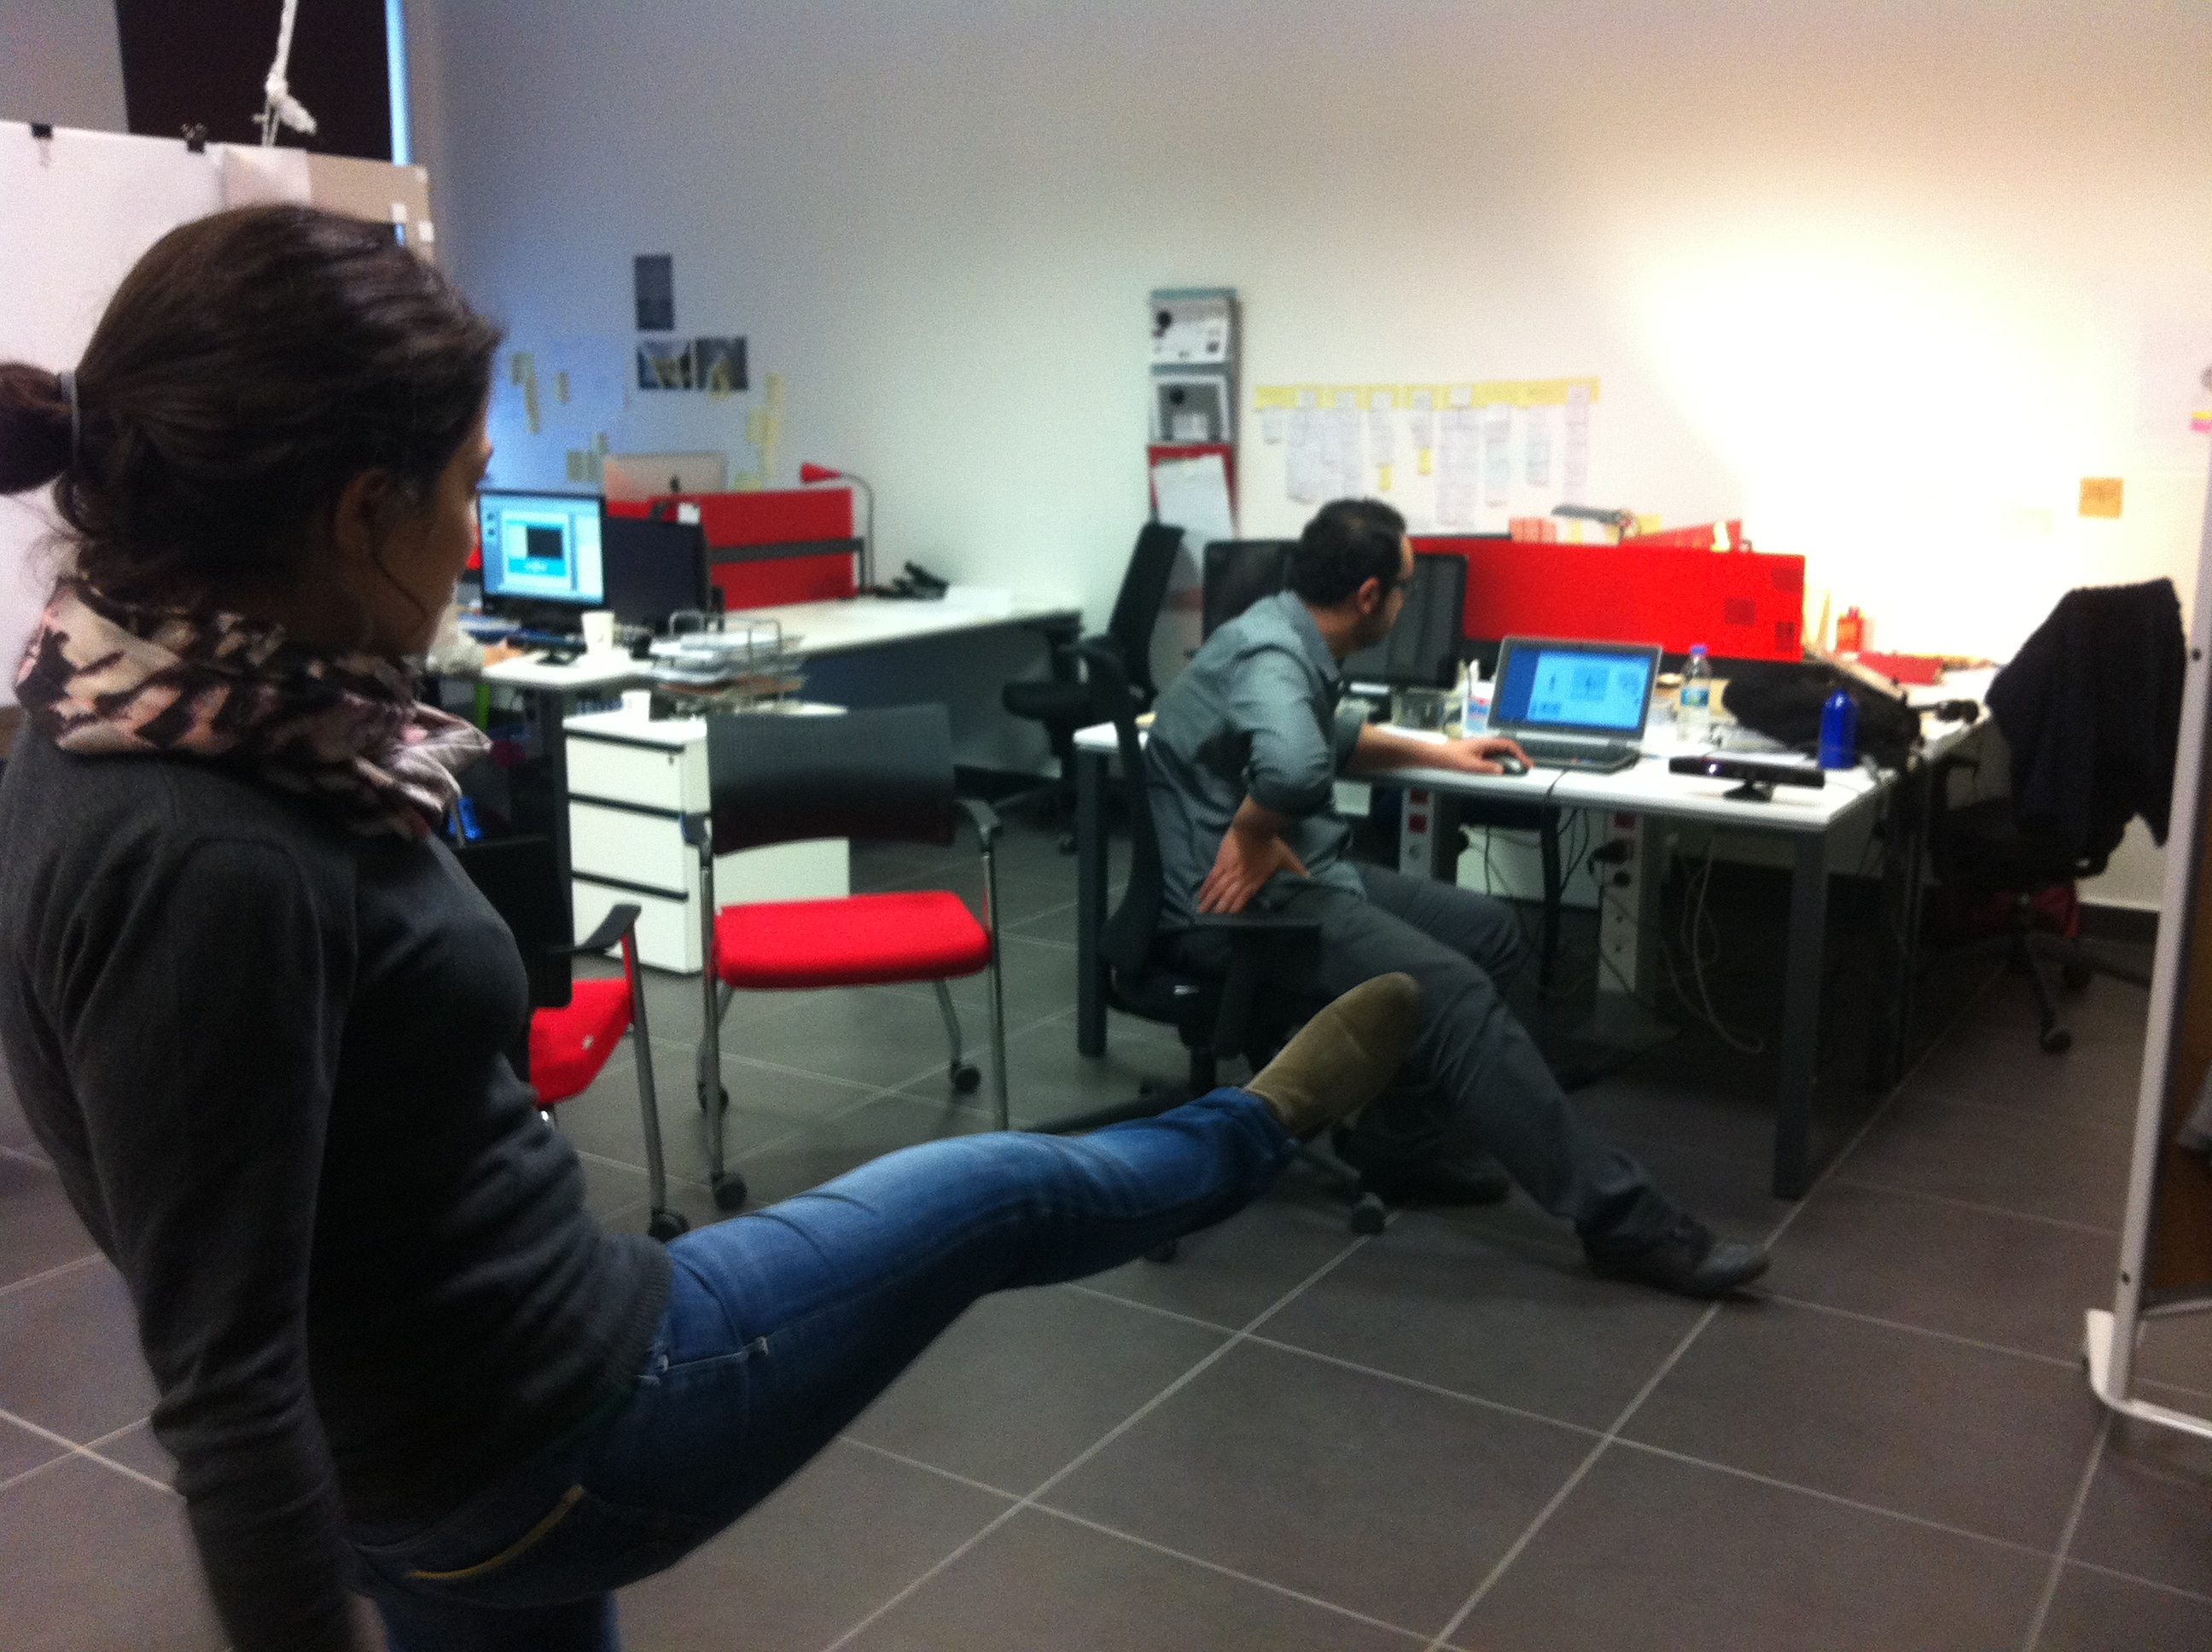
\includegraphics[width=.5\textwidth]{football}
\caption{User strategies included working in pairs. One user performs gestures in front of the sensor while the other marks hotspots that correspond to limb positions.}
\label{fig:football}
\end{SCfigure}

When working in pairs rather than alone, users adopted a different strategy when editing gestures: A single user would mark hotspots using the static on-screen silhouette of a human body as a reference and then test using the interactive representation. Working in pairs, one of the users preferred to stand in front of the sensor and perform gestures, while the other watched the moving representation on the screen and used it as a reference when marking hotspots (Figure~\ref{fig:football}). To allow a single user to enjoy the advantages of using the interactive skeletal model for authoring, future work can implement the ability to infer hotspots from demonstration, along with voice control to interact with the program from a distance (see Section~\ref{sec:future-work}).

Participants were interviewed after the study, where they suggested that while editing, being able to see where hotspots belonging to previously authored gestures reside could be beneficial. This visualization was later added into the Editor module in a later version of Hotspotizer.

\subsection{Generalizable Observations}

During the summative studies, observations that are relevant for the design of mid-air gestural interfaces in general were encountered.

Users who self-reported little experience with mid-air gestural interfaces (a vast majority among participants) tended to be unaware of the limitations regarding the sensor’s field of view. This manifested as an initial tendency to stand too close to the sensor and perform gestures in areas outside the sensor’s field of view. Within minutes, users adjusted to become aware of the boundaries of the interaction area. To promote users' awareness of the depth sensor's field of view, the depth map provided by the sensor could be displayed on screen, as opposed to displaying the user's skeleton alone.

As they tested and used their own gesture-controlled designs, users tended to keep the Hotspotizer interface open and utilize the on-screen representation of the human skeleton. This confirms that the requirements for including a tight feedback loop and a representation for reporting the user’s actions within space are justified. Based on this observation, I can recommend that interfaces based on mid-air gestures include a representation of the tracked skeleton(s).

In general, when designing gestures, users preferred to start with static poses or specify only the end point of a gesture trajectory, utilizing only one frame to implement their designs. In simple cases, such as in controlling the side-scrolling platformer, these designs did suffice. However, as the quantity and complexity of gestures in the interface increases, this approach results in a high number \emph{false positives} in gesture recognition due to intermediate movements intersecting hotspots. Users, due to inexperience, did not anticipate this. Through trial and error, gesture designs were revised and conflicts were resolved, by adding frames and authoring \emph{movement} further constrain designs. Often, gesture designs resulted in \emph{false negatives} due to spatially overconstrained designs that involved small volumes, requiring precise and accurate performance of gestures. Participants, through trial and error, revised their designs by enlarging hotspotized \emph{volumes} to allow for some degree of ambiguity when performing gestures. The general tendency among users was to initially design gestures that were temporally or \emph{sequentially underconstrained} and \emph{spatially overconstrained}. Designs that minimize conflicts by \emph{introducing sequential constraints} (i.e. more frames) while allowing for some flexibility by \emph{relaxing spatial constraints} (i.e. more hotspots) were observed to be more conducive to robust recognition (see Figure~\ref{fig:constraints}).

\begin{SCfigure}[\sidecaptionrelwidth][ht]
\centering
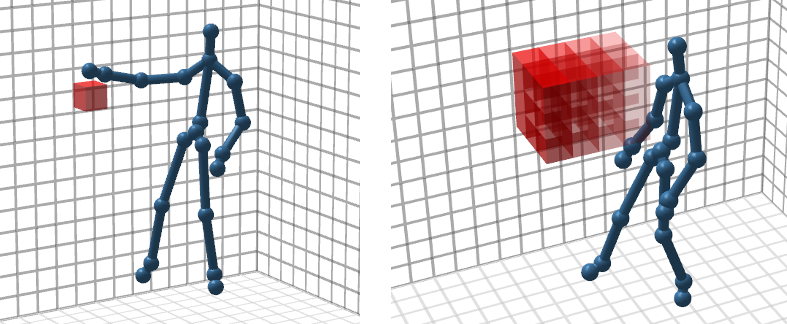
\includegraphics[width=.5\columnwidth]{constraints}
\caption{Initially, users preferred gesture designs that involved small hotspots and unspecified motion. Frames were added to constrain motion, and hotspots were enlarge to allow for variations during gesturing. Here, both panes depict hotspot configurations that may be used for a "punch" gesture. The configuration on the right is more conducive to robust recognition because of its sequentially constrained and spatially relaxed nature, compared to the rather extremely simplistic design on the left.}
\label{fig:constraints}
\end{SCfigure}